\documentclass{standalone}
\usepackage{tikz, pgfplots, amsmath}

\begin{document}
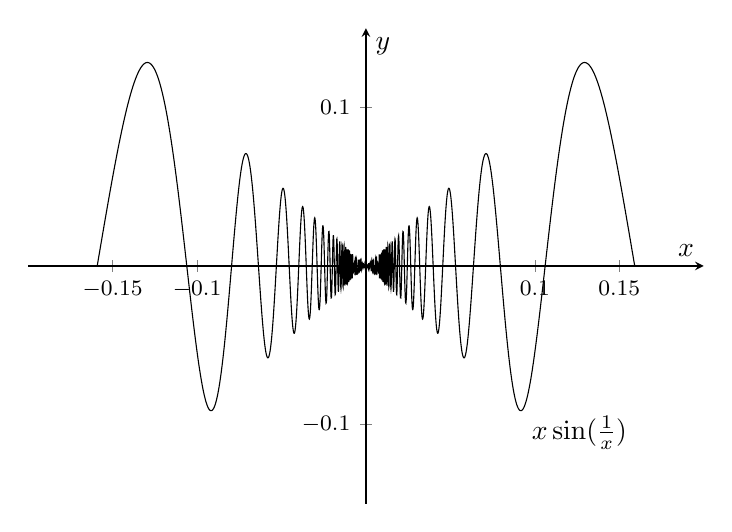
\begin{tikzpicture}
  \begin{axis}[
    thin,
    xtick={-0.15, -0.1, 0.1, 0.15},
    axis lines=middle, 
    xlabel=\(x\), 
    ylabel=\(y\), 
    tick label style={font=\footnotesize},
    width=4in, height=3in, 
    xmin=-0.2, xmax=0.2, 
    ymin=-0.15, ymax=0.15
    ]
    \addplot[blue, domain={-1/(2*pi)}:{1/(2*pi)}, samples=2000, smooth, black]{x * sin(deg(1/x))};
  \end{axis}
    \node at (7, 0.9) {\(x \sin(\frac{1}{x})\)};
\end{tikzpicture}
\end{document}
